\chapter{Results and Discussion}

\section{Camera Network}
Camera Network provided a great asset in acquiring the relevant dataset. The system is aimed at real-time processing of multiple camera feed. However, minor steps backs are faced during the footage capture. The support for network is maintained by a Chinese video surveillance manufacturer, abbreviated as UNV. The software interface have lower support for live streaming of footage, which leads to complex method of acquiring frame. The camera occasionally provides with corrupted frames (see figure \ref{fig:corrupted}), leading to false detection. Camera footage is extracted at 25 FPS, $1920*1080$ px.

\begin{figure}[!ht]
	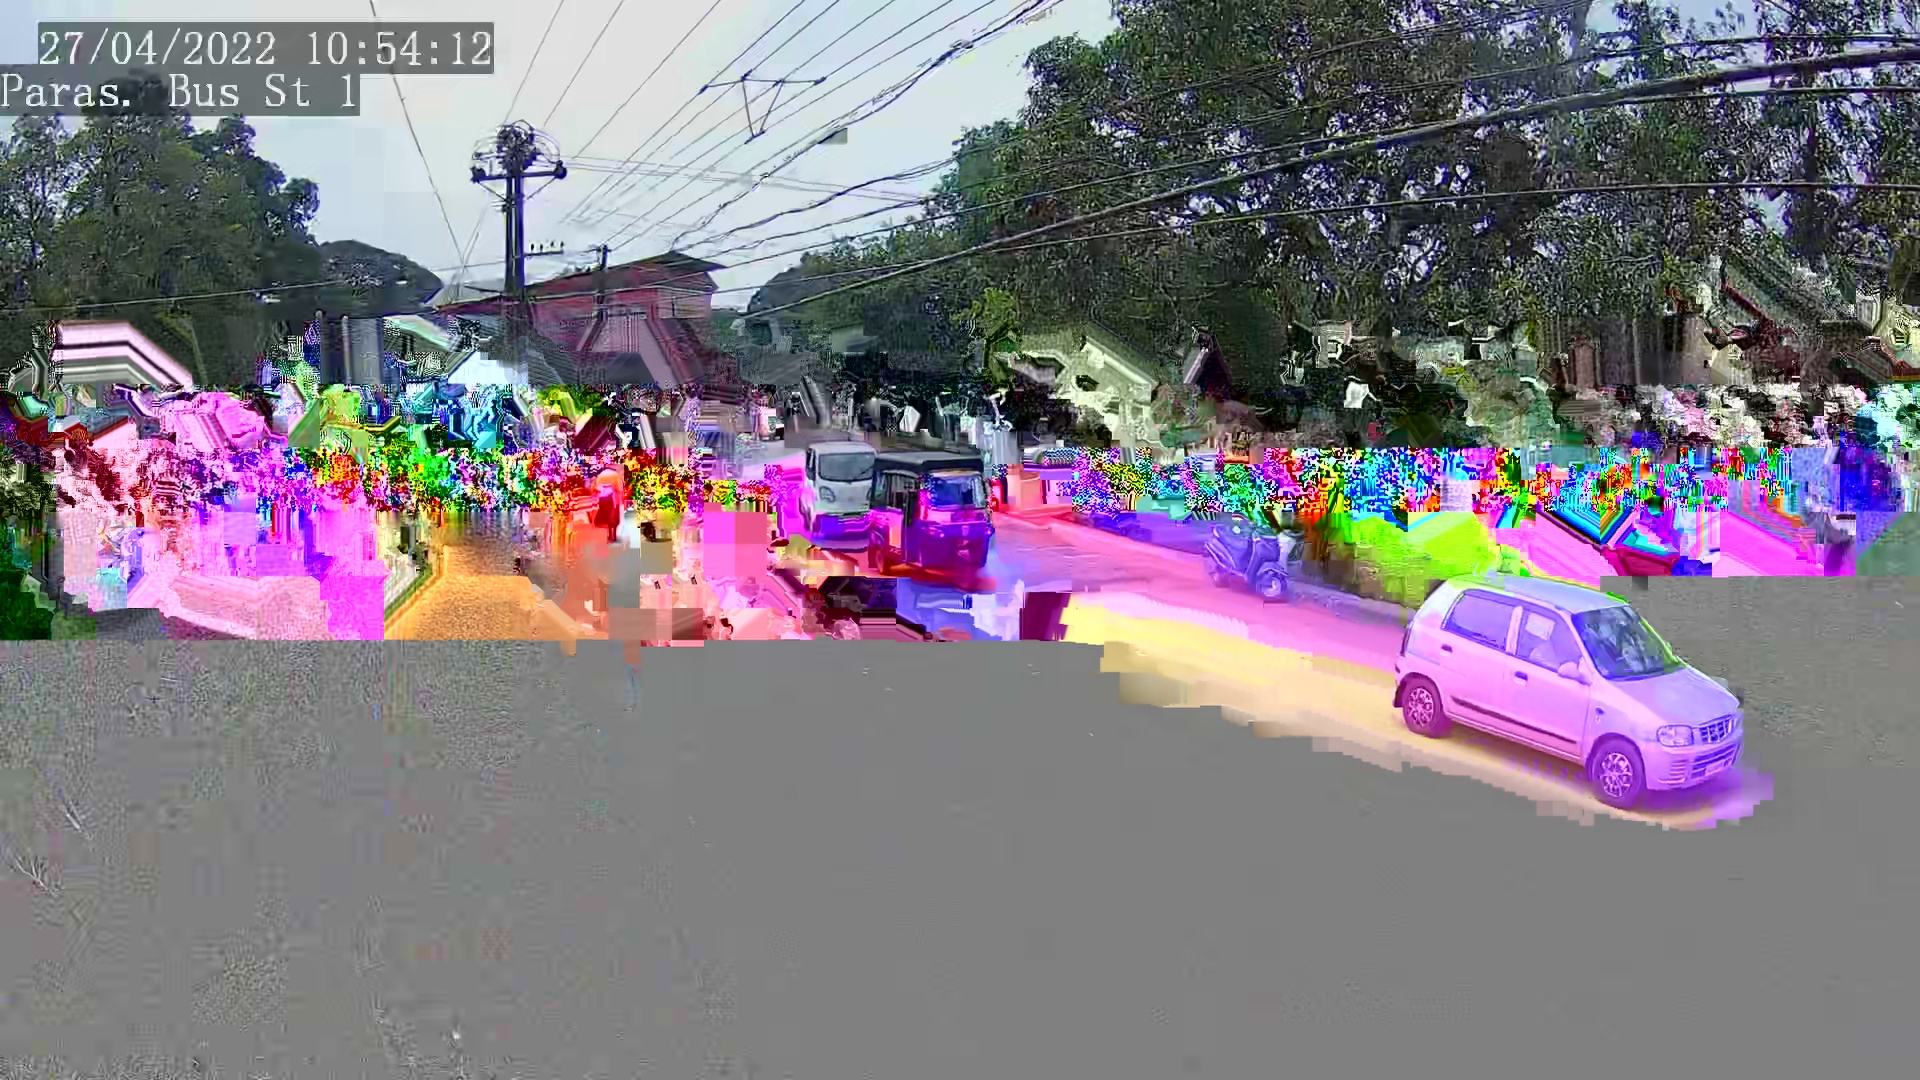
\includegraphics[width=0.32\linewidth]{Images/camera_footage/corrupted1} \hfill
	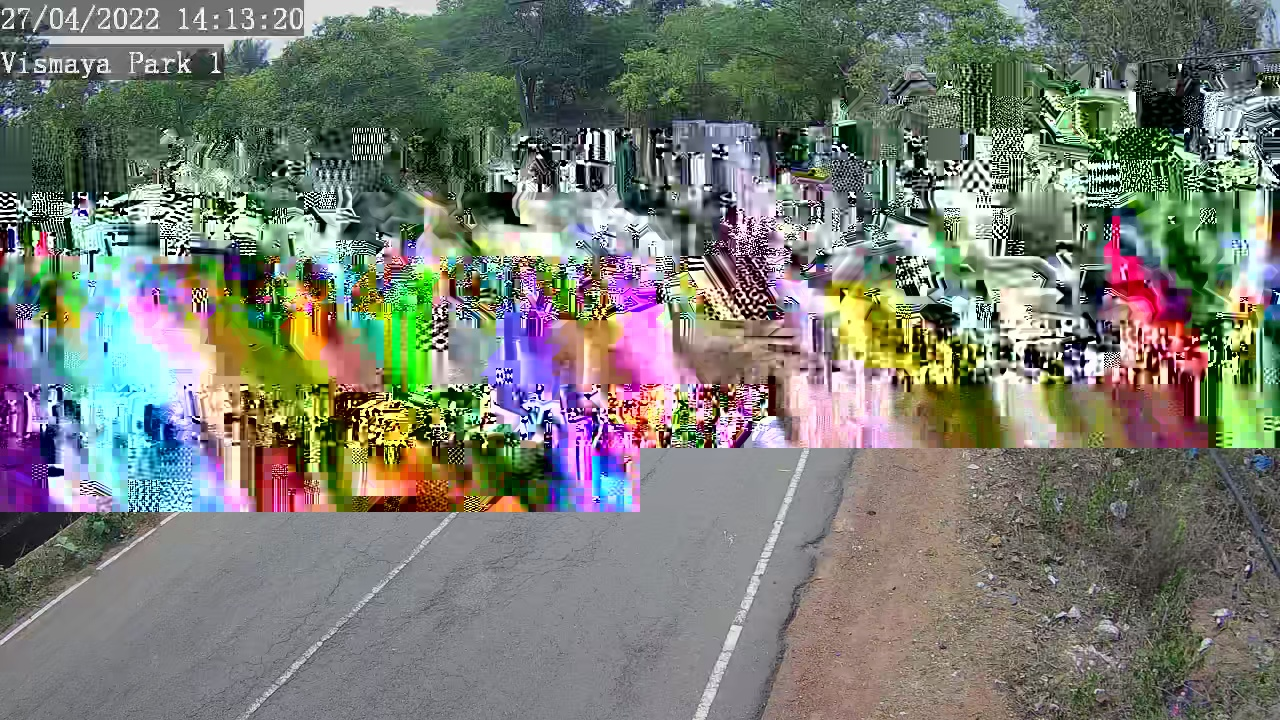
\includegraphics[width=0.32\linewidth]{Images/camera_footage/corrupted2} \hfill
	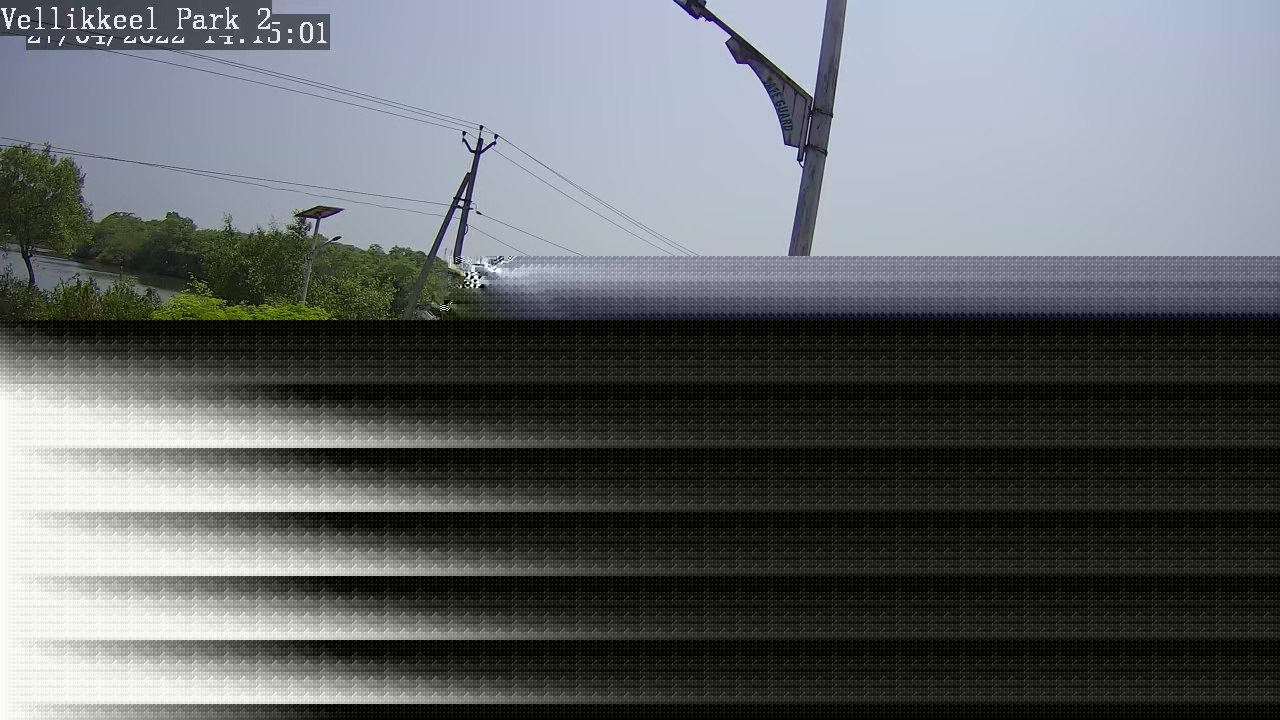
\includegraphics[width=0.32\linewidth]{Images/camera_footage/corrupted3} \\ 
	\\
	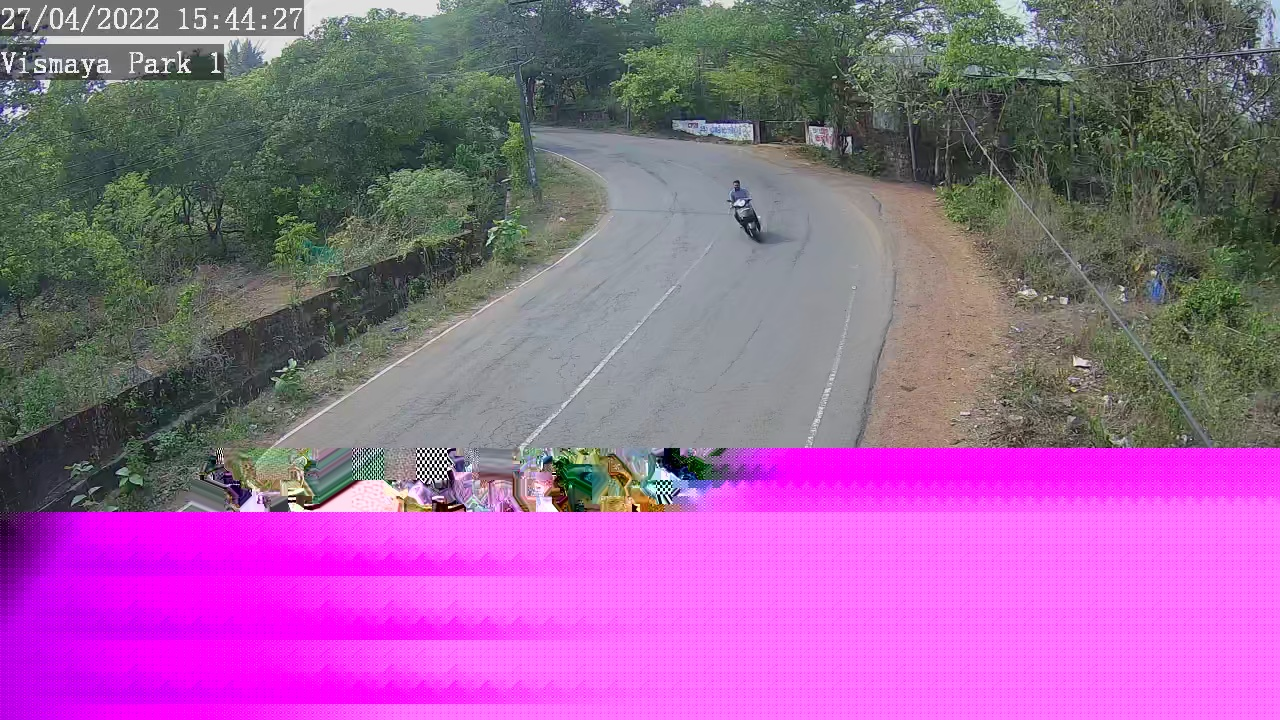
\includegraphics[width=0.32\linewidth]{Images/camera_footage/corrupted4} \hfill
	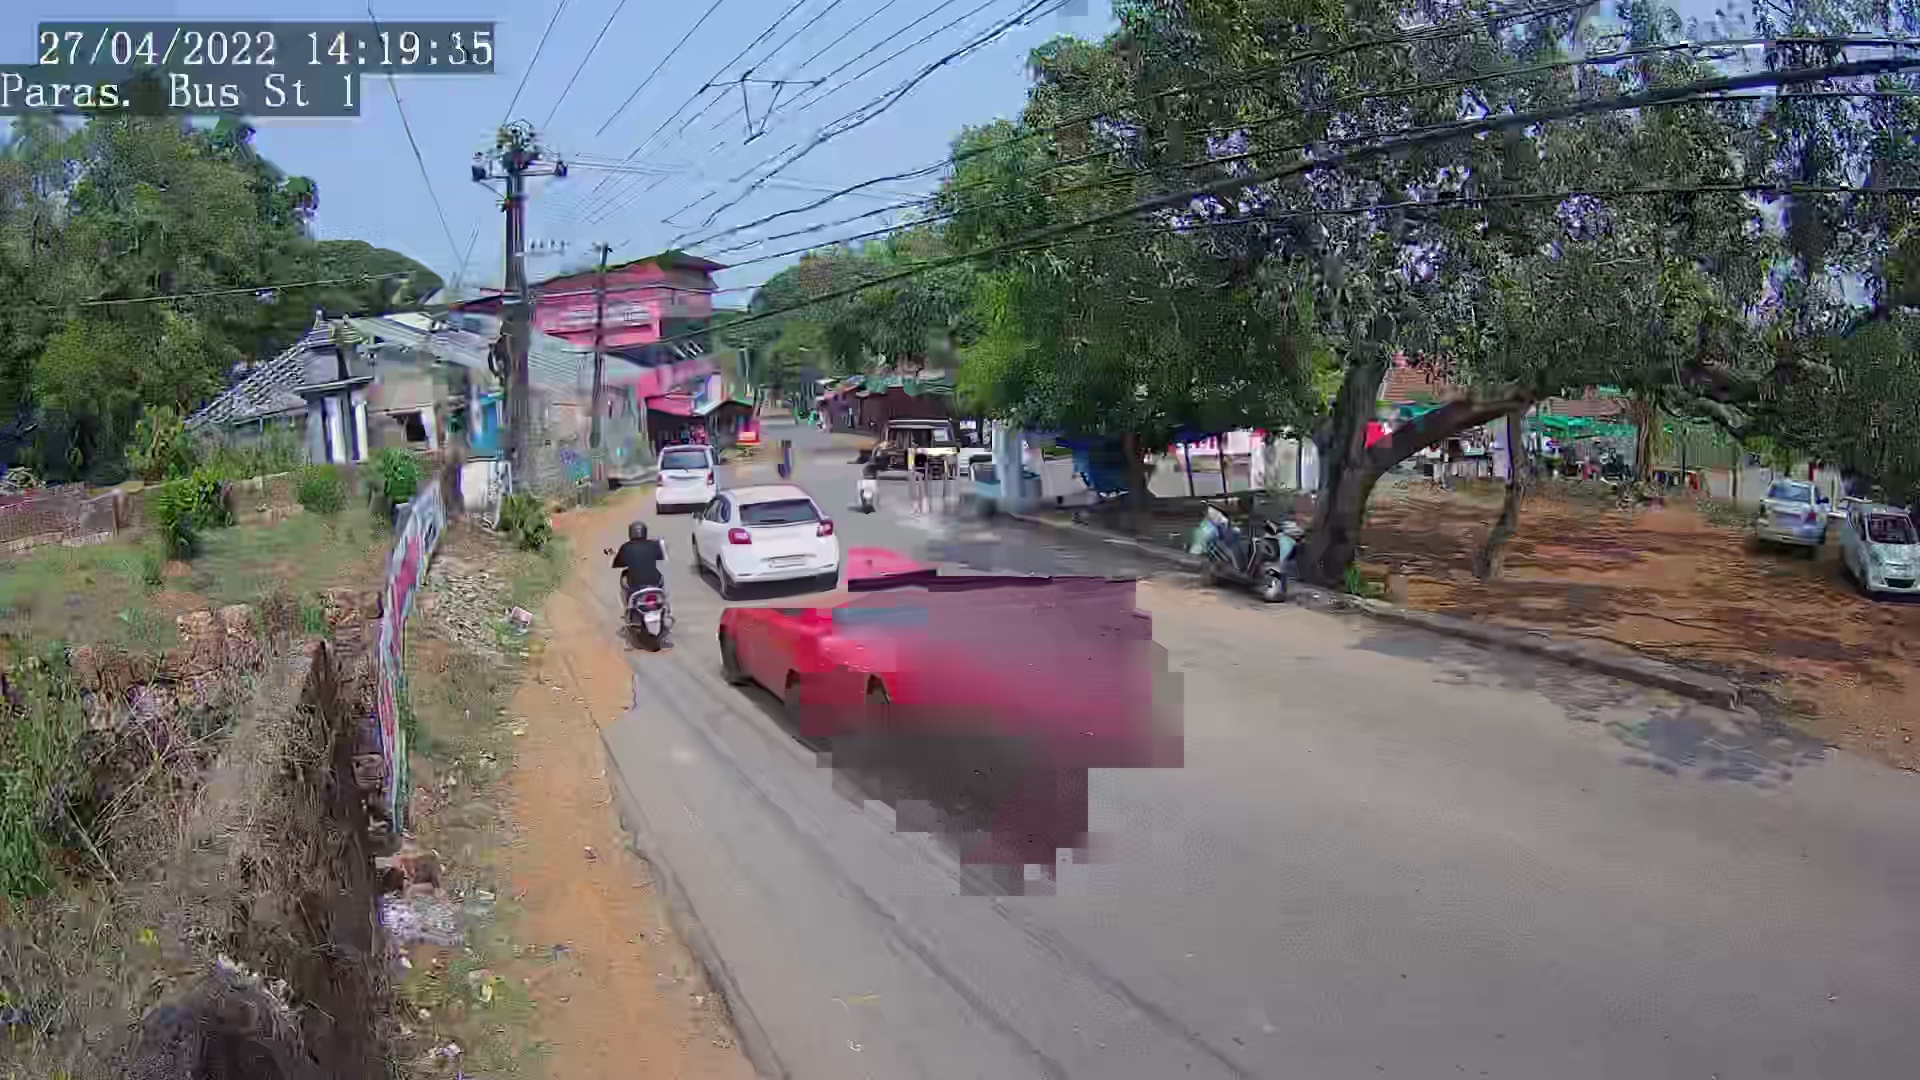
\includegraphics[width=0.32\linewidth]{Images/camera_footage/corrupted5} \hfill
	
\includegraphics[width=0.32\linewidth]{Images/camera_footage/corrupted6} 
	\caption{Corrupted Camera footage}
	\label{fig:corrupted}
\end{figure}

\section{YOLOv4}
YOLOv4 model is trained with 1559 images for 9 classes as illustrated in table \ref{tab:dataset_sum1}. Model accuracy is easy calculated by Darknet and is shown in table \ref{tab:yolo_matrix} and \ref{tag:yolo_score}. The model, in the deployment ran at slower speed of about 19.1 FPS. The decrease in speed is due to the unwanted processing of dead/corrupted frame. Speed can also be improved by reducing the yolo network size, compromising accuracy.

\begin{table}[!ht]
	\centering
	\begin{tabular}{|l|l|l|l|}
		\hline
		Class label    & True Positive & False Positive & Avg Precision \\ \hline
		auto           & 424           & 38             & 98.25\%       \\ \hline
		bus            & 327           & 42             & 99.57\%       \\ \hline
		tempo traveler & 76            & 7              & 97.12\%       \\ \hline
		tractor        & 130           & 2              & 98.44\%       \\ \hline
		truck          & 516           & 33             & 99.28\%       \\ \hline
		van            & 227           & 22             & 98.14\%       \\ \hline
		two wheeler    & 770           & 241            & 91.62\%       \\ \hline
		car            & 644           & 91             & 96.99\%       \\ \hline
		jcb            & 0             & 0              & 100.00\%      \\ \hline
	\end{tabular}
	\caption{YOLOv4 accuracy matrix}
	\label{tab:yolo_matrix}
\end{table}

\begin{table}[!ht]
	\centering
	\begin{tabular}{|l|l|}
		\hline
		Precision            & 87\%    \\ \hline
		Recall               & 96\%    \\ \hline
		F1-score             & 91\%    \\ \hline
		True Positive        & 3114    \\ \hline
		False Positive       & 476     \\ \hline
		False Negative       & 134     \\ \hline
		Avg IoU              & 72.13\% \\ \hline
		Mean Avg precision   & 97.71\% \\ \hline
		Total Detection Time & 1166 Seconds \\ \hline
		Detection count      & 12349 \\ \hline
		Unique truth count   & 3257 \\ \hline
	\end{tabular}
	\caption{YOLOv4 evaluation}
	\label{tag:yolo_score}
\end{table}

\begin{figure}[ht!]
	\centering
	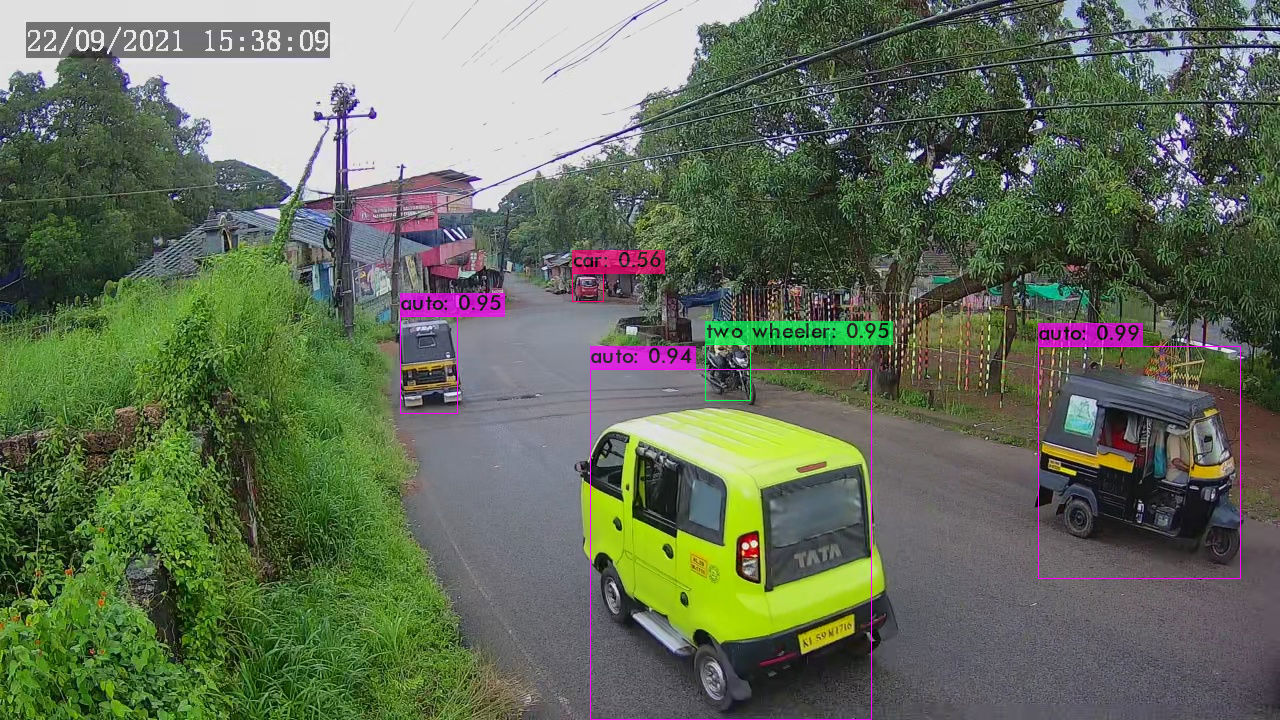
\includegraphics[width=0.8\linewidth]{Images/predictions}
	\caption{YOLOv4 vehicle predictions}
\end{figure}



\section{DeepSORT}
Ground Truth dataset was not available to quantize the result. However, via visual inception, it was found that the model was able to assign correct ID number to most of the vehicles. I was observed that such an increase in accuracy was observed due to the presence of Kalman filtering algorithm. The deep matrix association for humans was trigger only at the presence of humans. It lead to a mismatch where traditional Kalman filter tries to re-Id the bounding boxes, where as deepSORT tries to match human description leading to wrong answer. The anomaly can be strongly seen in public transport bus. Building of deep matrix for vehicle can improve the system.

\subsection{Siamese Network}
Proper Siamese Network was unable to construct, as the layers of yolov4 models was not able to selectively extract. The YOLOV4 model have tight coupling between layers, with multiple output and input vectors. The model is originally implement in Darknet.  This provided hindrance during the extraction of layers using keras and python. Ground Truth dataset is not able to quantize its accuracy



